% Sample file for AES paper
\documentclass{aes2e}

% Metadata Information
\jyear{2010}
\jmonth{October}
\jvol{1}
\jnum{1}


\begin{document}

% Page heads
\markboth{A1LASTNAME AND A2LASTNAME}{semantical analysis of open band}

% Title portion
\title{analysis of the Open Band\thanks{To whom correspondence should be addressed Tel: +1-240-381-2383; Fax: +1-202-508-3799; e-mail: info@schtm.org}}

%Author Info.
\authorgroup{
\author{A1FIRSTNAME A1LASTNAME},
\role{AES Member}
AND \author{A2FIRSTNAME A2LASTNAME},
\role{AES Fellow}
\email{(abc@abc.com)\quad\quad\quad\quad\quad\quad\quad\quad\quad\quad\quad\quad (xyz@abc.com)}
\affil{Universityxyz, City, Country}
}

%Abstract
\abstract{%
Open Band was developed as a research project in audience participatory performance and has been presented in some festivals and conferences since 2016. The project was based on a chat interface, where the audience could anonymously input messages, that were converted into sound and played in a collective performance. As result of this performances, we have audio and screen recordings and also logs of the messages sent by the users in several different contexts. In this paper, we will analyze the content of this performances to discuss results of implications of the project. For that, we will make some semantical analyses and use as well automatic tools for natural language processing.}


\maketitle

%Head 1
\section{INTRODUCTION}

Audience participatory performance is been a recurrent topic throughout music and technology and contemporary arts discussions. In contrast to presentational performances, where there's a strict division between audience and performers, participatory performances tries to blur the limits \cite{kattwinkel2003audience} between audience and the the performers  \cite{kattwinkel2003audience}.  In Brazilian arts, this is been discussed since Helio Oiticica's "Parangoles", weareable pieces for playing through dance, and Ligya Clark's movable sculptures "Bichos"\cite{Braga2008}. 

Today, developments in technology brings lots of resources to facilitate and encourage participation in performances and installations such as analog to digital conversors as Arduino, different kinds of sensors, ubiquitous computing and new programming languages and frameworks. In an ideal application of such nature, participants are able of interacting and these interactions create sensible influence to the performance environment, taking each participant as a creator, player or agent, such as audience and actors are the same, one only group\cite{Wu2017}.

Designing collaborative environments can be challenging. Open Band is one attempt of exploring this. We use music as our domain as music is known for its social functions of cohesion and communication \cite{Koelsch:2014}. The idea was to to build an ``open" Work as defended by Umberto Eco\cite{eco_obra_2015}, which, according to Robey in \cite{eco_obra_2015}, require of the public \textit{``a much greater degree of collaboration and personal involvement than was ever required by the traditional art of the past."},In Open Works, it is \textit{``the artist's decision to leave the arrangement of some of their constituents either to the public or to chance, thus giving them not a single definitive order but a multiplicity of possible orders"}.

were the final arrangement and form is given to the public to give shape.

We tried to create something that could easily be used as a kind of musical instrument by anyone independent of any previous knowledge of music. Musical instruments in general can be expensive or too complex to manipulate, so we seek for use web technologies as media to develop the interface, as they are easy to program \cite{Roberts2013webbrowser}, don't require installation \cite{Wyse2013viability}, are ubiquitous and easy to distribute \cite{lee_web-based_2015}, as pointed by many researchers. We choose typing as method of input  Our web-based instrument has been used to create experimental participatory music performances where everyone in the audience can join through its cell phone, tablet or laptop, and can playing through typing. 

As for now, some data for past performances has been obtained, a concern on what kind of interaction is happening has been growing. Although not simple, trying to find out or measure engagement from recorded messages is desired. Also, recurrent themes or linguistic features can be found, and there is interesting describing that.

%One of the things that can keep people away from music is a poor access to musical instruments, that can be too expensive and with too complex manipulation. Many researches point to Web Audio technology as base for developing more accessible audio interfaces \cite{Roberts2013webbrowser}, as they don't require installation, are ubiquitous and easy to distribute \cite{lee_web-based_2015}, and can easily be applied to construct interactive systems, independent of any extra software installation \cite{Wyse2013viability}. 

%For this project we are trying to build an "open" work as defended by Umberto Eco \cite{eco_obra_2015}, a work in movement, that can be shaped by each participant, as well as developing a web-based instrument, to be used in an experimental music performance where everyone in the audience can join through its cell phone, tablet or laptop, that can be played through typing, an input method familiar to every user of modern devices. Instead of individual actions, everything typed is played on every connected device, potentializing  volume on the available speakers..

\section{Background of the Project}
The project begun as a proposal for some of the NuSom colaboration The first performance, at Bigorna festival, was in a public square close to Avenida Paulista, in a experimental music festival organized by Estudio Fita Crepe in collaboration with the NuSom research group, were invited musicians were playing on a stage, intercalated with NuSom proposed projects. In the research group, we propose to think in some performances that could explore the physical space of the square. One of the proposed projects was a collaborative electronic improvising session, made by Victor Kisil's student of Music Production at University Anhembi Mourumbi (UAM), the same group of students collaborated with the Open Band Project, sending some samples to build one of the samples pack used (Samples2). So they were really engaged into the performance and were also the majority of the public present.


\section{Numerical Analysis of Performances}

\subsection{Evaluated performances}

To analyze the Open Band project, we took data from the 4 first public performances of the project, that occurred in Brazil on the second semester of 2016. In commons, they were all using mostly the same version of the software, with some minor changes mostly for bug fixes and they happened with text in Portuguese:
\begin{arabiclist}
\item{}Bigorna Festival, 26 of June.
\item{}IV Congresso da ABRAPEM - Congress of the Brasilian Association of Musical Performance, 30 of june.
\item{}Computer Music Concert at IME - Institut of Mathematics and Statistics - 22 of september.
\item{}Áudio InsurgIencia Festiva - 8 of october.
\end{arabiclist}



The second performance was presented at ABRAPEM Congress, an academic meeting of professional and mostly traditional musicians. There were less people on the audience and the space was a traditional conference hall, with stage, were the chat was projected, and chairs were the audience of about 23 people seated. 

\begin{figure*}
\centering
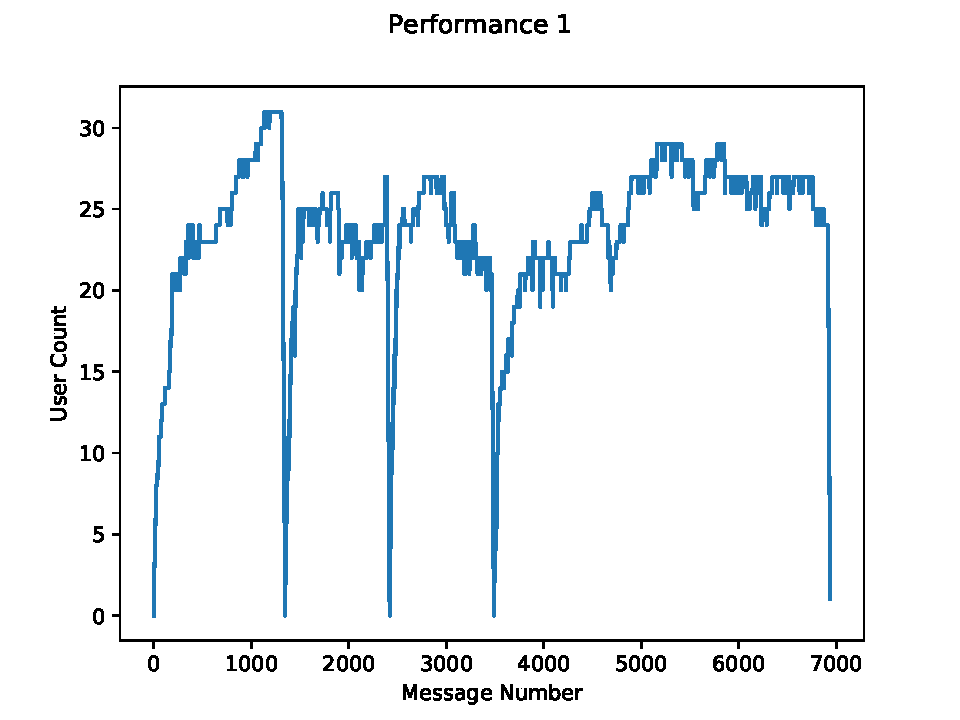
\includegraphics{num_analysis/p1_us.pdf}
\caption{User count for the first performance. The x-axis represents the message number in the log.}
\end{figure*}

- bigorna Festival - 26 june
- Festival of ABRAPEM - 30 june
- Concerto de Computaçao musical no IME - 22 sepetember
- 8 october - Audio Insurgência


\subsection{Character usage}

Table shows the 30 most used characters over content of written messages. For each of these characters, a count number that represents the overall number of appearances for the character, and a frequency number that shows relation between the count of the character and the global number of characters for written messages. The results differentiate upper and lowercase characters, as it had different behavior for the performance.

As the main language used in latter performances was portuguese, some character usage follows patterns found in that language. Some unexpected behavior was presence of character '.' with 1.99\% frequency, with correspond to the kick bass sample, 'P' with 1.01\%, ';' with 0.96\%, and ')' with 0.81\%.

\begin{figure*}
\centering
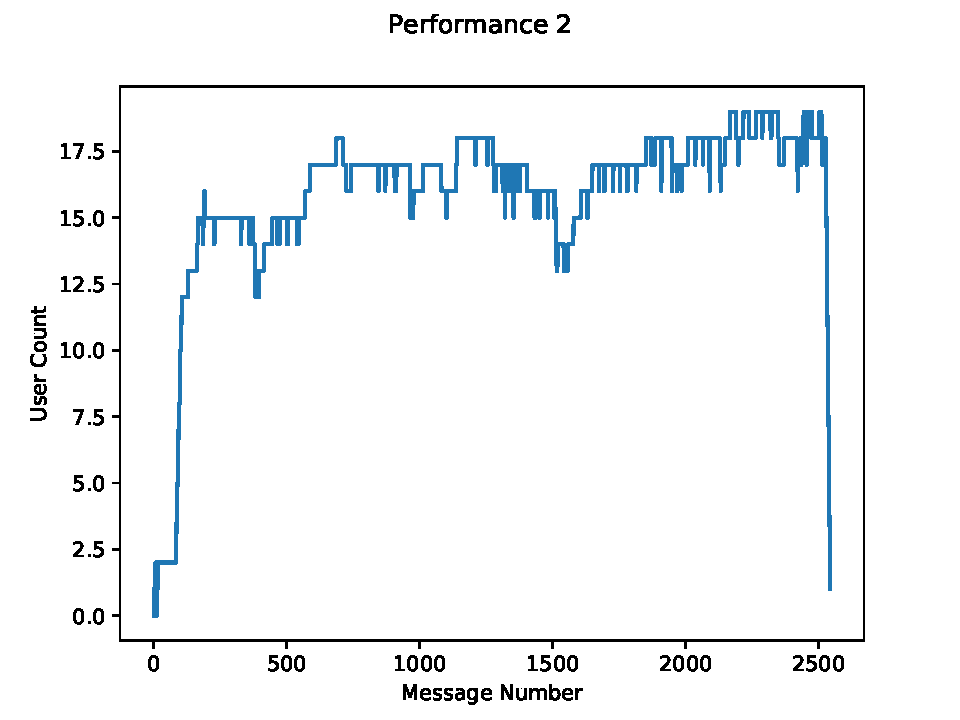
\includegraphics{num_analysis/p2_us.pdf}
\caption{User count for the second performance. The x-axis represents the message number in the log.}
\end{figure*}

\begin{table}
\tabcolsep8.1pt
\tbl{30 most used characters}{%
\begin{tabular}{@{}lcc@{}}
frequency & count & character \colrule\toprule
  9.32\%&		6863&           	a\\                   
  6.18\%&		4551&           	o\\                   
  5.81\%&		4282&           	e\\                   
  4.57\%&		3366&           	i\\                   
  3.76\%&		2772&           	s\\                   
  3.63\%&		2671&           	r\\                   
  3.43\%&		2527&           	u\\                   
  3.14\%&		2314&           	t\\                   
  2.76\%&		2033&           	n\\                   
  2.70\%&		1991&           	m\\                 
  2.52\%&		1859&           	d\\                 
  2.24\%&		1647&           	l\\                 
  2.09\%&		1542&           	h\\                 
  2.04\%&		1504&           	c\\                 
  1.99\%&		1466&           	.\\                 
  1.86\%&		1367&           	A\\                 
  1.54\%&		1135&           	p\\                 
  1.33\%&		978 &           	k\\                 
  1.09\%&		805 &           	O\\                 
  1.08\%&		797 &           	b\\                 
  1.01\%&		747 &           	P\\                 
  1.01\%&		744 &           	g\\                 
  0.99\%&		732 &           	v\\                 
  0.98\%&		721 &           	f\\                 
  0.97\%&		713 &           	0\\                   
  0.96\%&		709 &           	;\\             
  0.89\%&		656 &  \textbackslash\\               
  0.84\%&		618 &           	S\\                 
  0.83\%&		615 &           	!\\                   
  0.81\%&		595 &           	)\\\botrule
\end{tabular}}
\begin{tabnote}
Quantitative data about the characters.
\end{tabnote}
\end{table}

\subsection{Word usage}

Table shows the 30 most used characters over content of written messages. For each of these characters, a count number that represents the overall number of appearances for the character, and a frequency number that shows relation between the count of the character and the global number of characters for written messages. The results differentiate upper and lowercase characters, as it had different behavior for the performance.

Besides some word usage following patterns found in Portuguese language, unexpected behavior found in messages was the presence of 'character words', that is, words or frases consisting of one only character. One hypothesis brought to explain this behavior is that people would usually experiment lone characters to hear those sounds.

\begin{table}
\tabcolsep8.1pt
\tbl{30 most used words}{%
\begin{tabular}{@{}lcc@{}}
frequency & count & word \colrule\toprule
  2.71\%&		409&            	o\\             
  1.98\%&		298&            	A\\                   
  1.56\%&		236&            	0\\                   
  1.24\%&		187&            	a\\                   
  1.23\%&		185&            	de \\                 
  1.13\%&		171&            	P  \\                 
  0.88\%&		133&            	m  \\                 
  0.84\%&		127&            	que\\                 
  0.78\%&		117&            	e  \\                 
  0.76\%&		114&            	f  \\                 
  0.70\%&		106&            	d  \\                 
  0.70\%&		105&            	5  \\                 
  0.68\%&		102&            	u  \\                 
  0.66\%&		100&            	O  \\                 
  0.64\%&		97&             	S  \\                 
  0.64\%&		97&             	ola\\                 
  0.64\%&		96&             	1  \\                 
  0.58\%&		87&             	n  \\                 
  0.55\%&		83&             	2  \\                 
  0.51\%&		77&             	do \\                 
  0.48\%&		73&             	thick  \\             
  0.45\%&		68&             	marquee\\             
  0.44\%&		67&             	da     \\             
  0.42\%&		64&             	3      \\             
  0.42\%&		63&             	no      \\            
  0.42\%&		63&             	E       \\            
  0.40\%&		60&             	interval\\            
  0.40\%&		60&             	eye     \\            
  0.39\%&		59&             	s       \\            
  0.34\%&		52&             	lps\\\botrule
\end{tabular}}
\begin{tabnote}
Quantitative data about the words.
\end{tabnote}
\end{table}

number of messages played:
performance 1: 2399
performance 2: 1411
performance 3: 1892
performance 4: 1620

number of messages sent:
performance 1: 1558
performance 2: 849
performance 3: 594
performance 4: 723

total number of tokens
1: 2836
2: 1615
3: 1764
4: 1494

words on dictionary
1: 404 (14\%)
2: 240  (52\%)
3: 292 	(52\%)
4: 358 (58\%)




%number of unique tokens:
%1: 1274
%2: 1110
%3: 960
%4: 822

%words on dictionary
%1: 415
%2: 376
%3: 341
%4: 325








First step was to remove the repeated messages, that were generated by clicking on an already sent message, to get only the messages typed



We also compared the the words used on performances with a Portuguese dictionary from Open Office (reference) of words in a python script, and we realized that in every performance, the majority of words are actually outside of the dictionary, so people tend 

https://www.wordclouds.com/

\begin{figure}
\centering
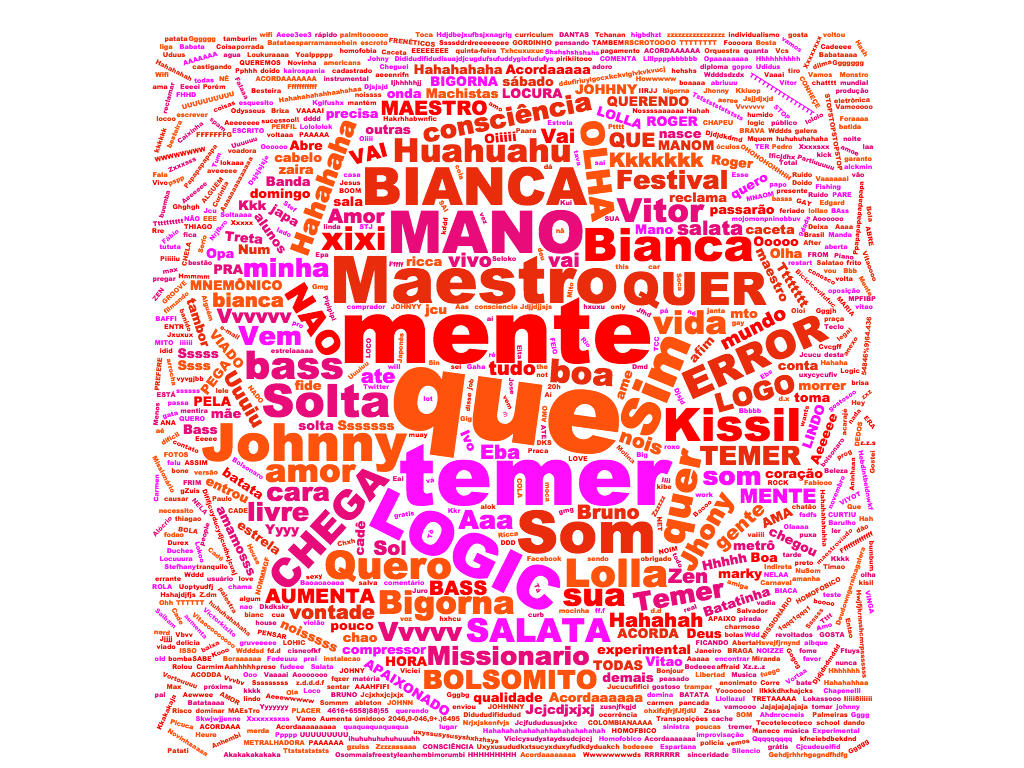
\includegraphics[width=1\linewidth]{img/wordcloud_performance1.png}
\caption{Tag cloud of the performance 1.}
\end{figure}

\begin{figure}
\centering
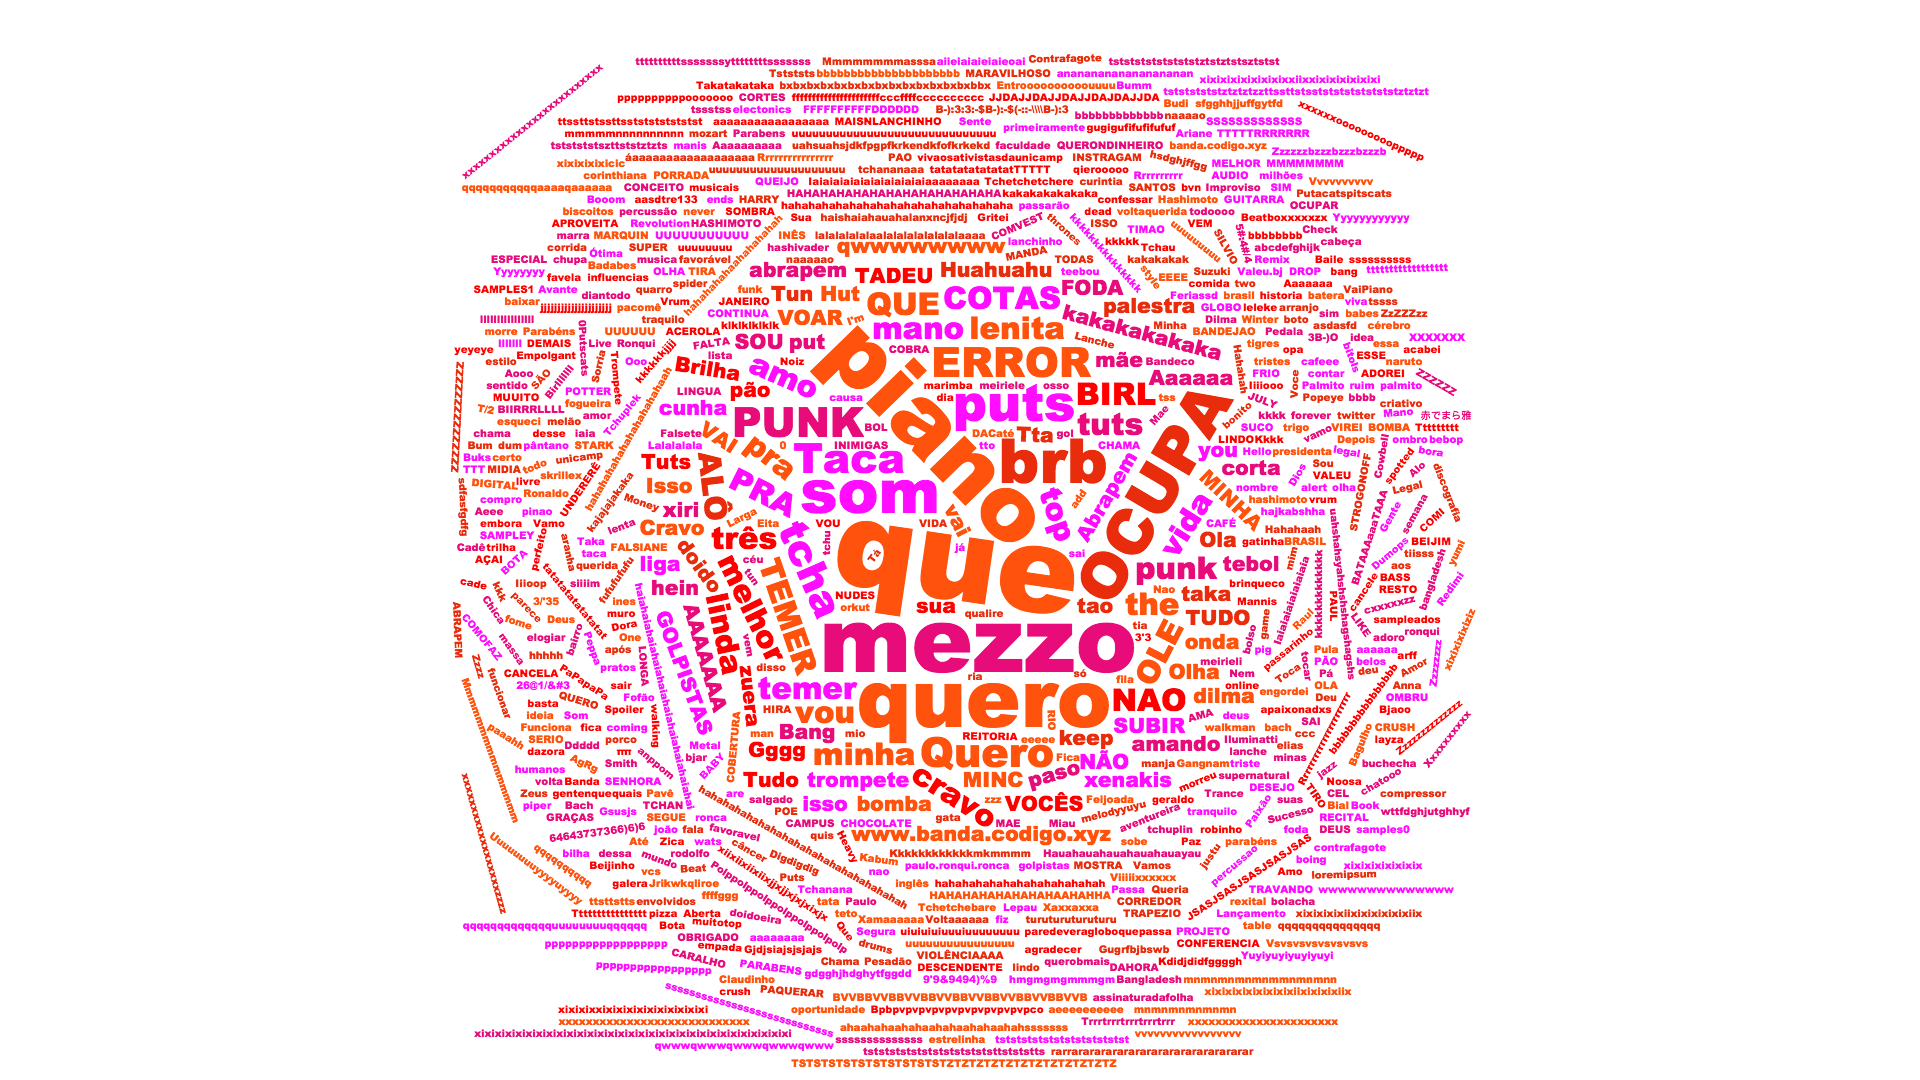
\includegraphics[width=1\linewidth]{img/wordcloud_performance2.png}
\caption{Tag cloud of the performance 2.}
\end{figure}

\begin{figure}
\centering
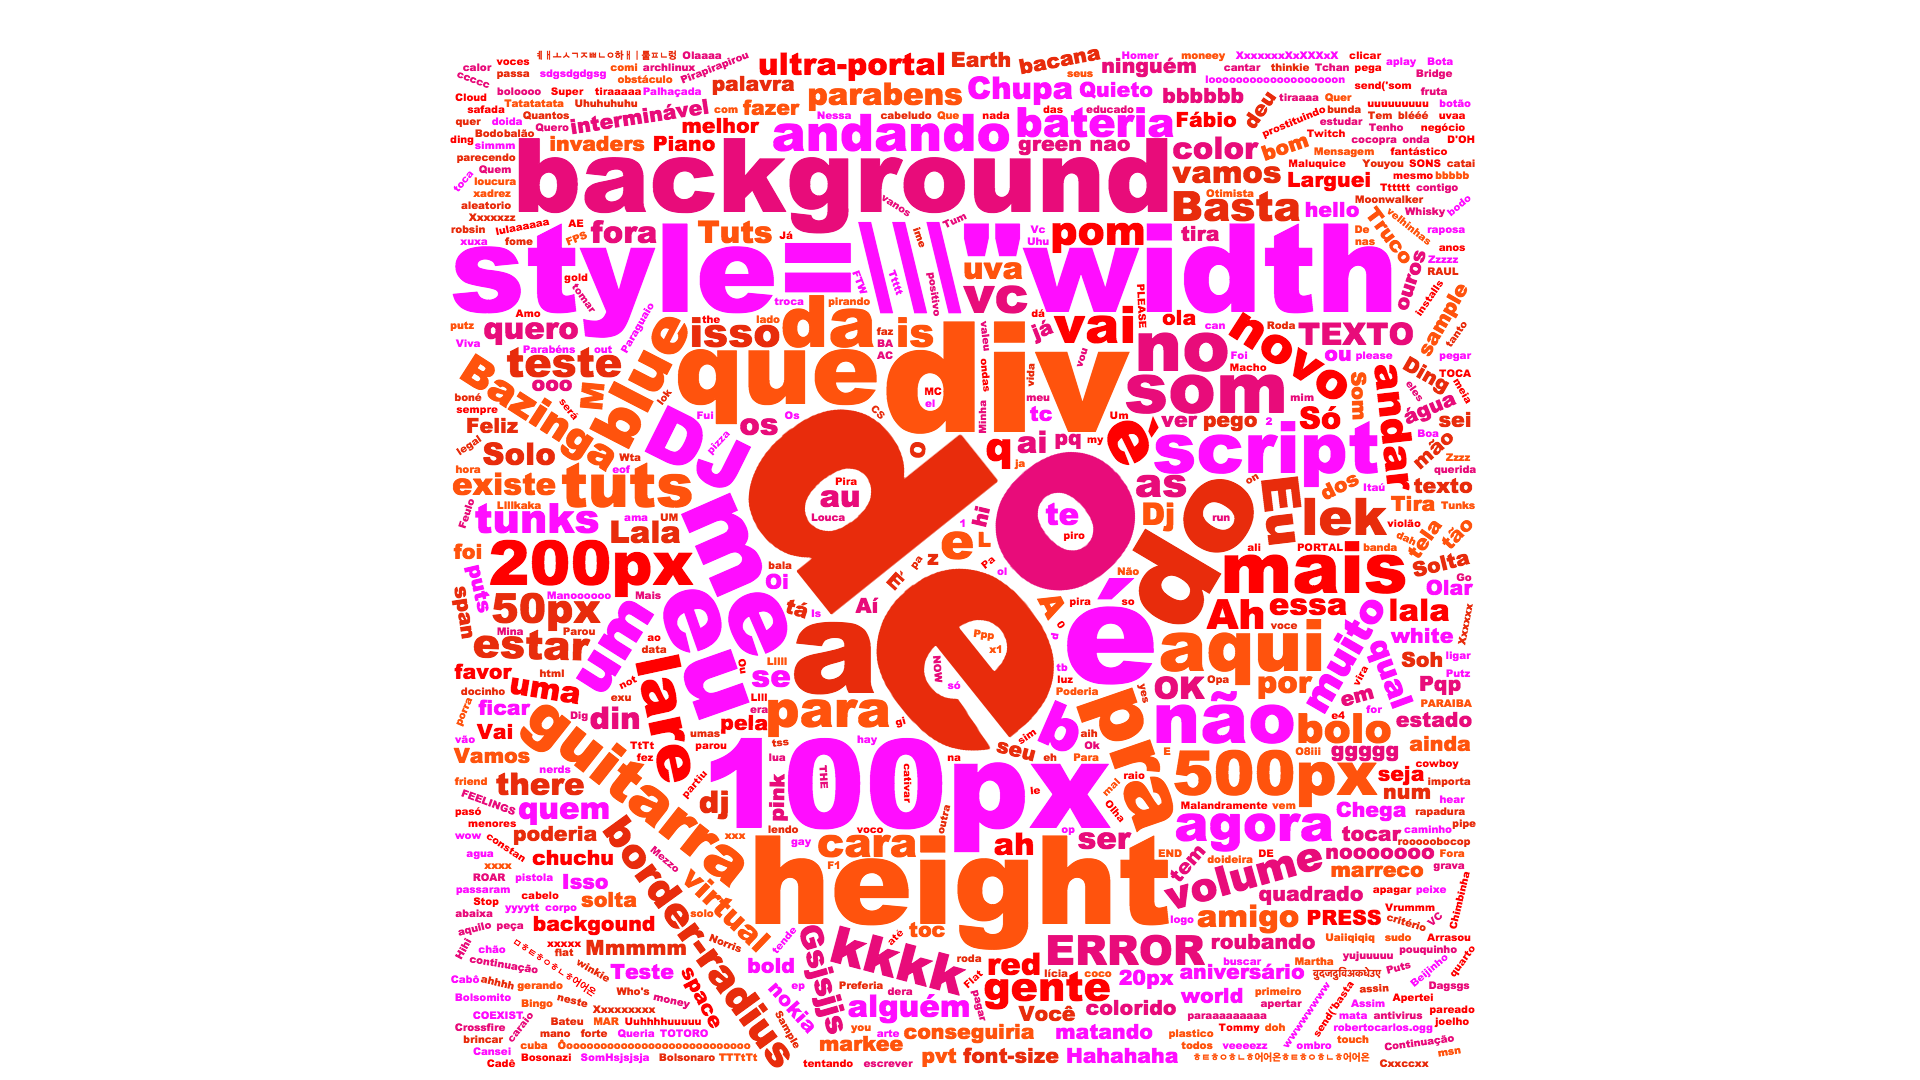
\includegraphics[width=1\linewidth]{img/wordcloud_performance3.png}
\caption{Tag cloud of the performance 3.}
\end{figure}

\begin{figure}
\centering
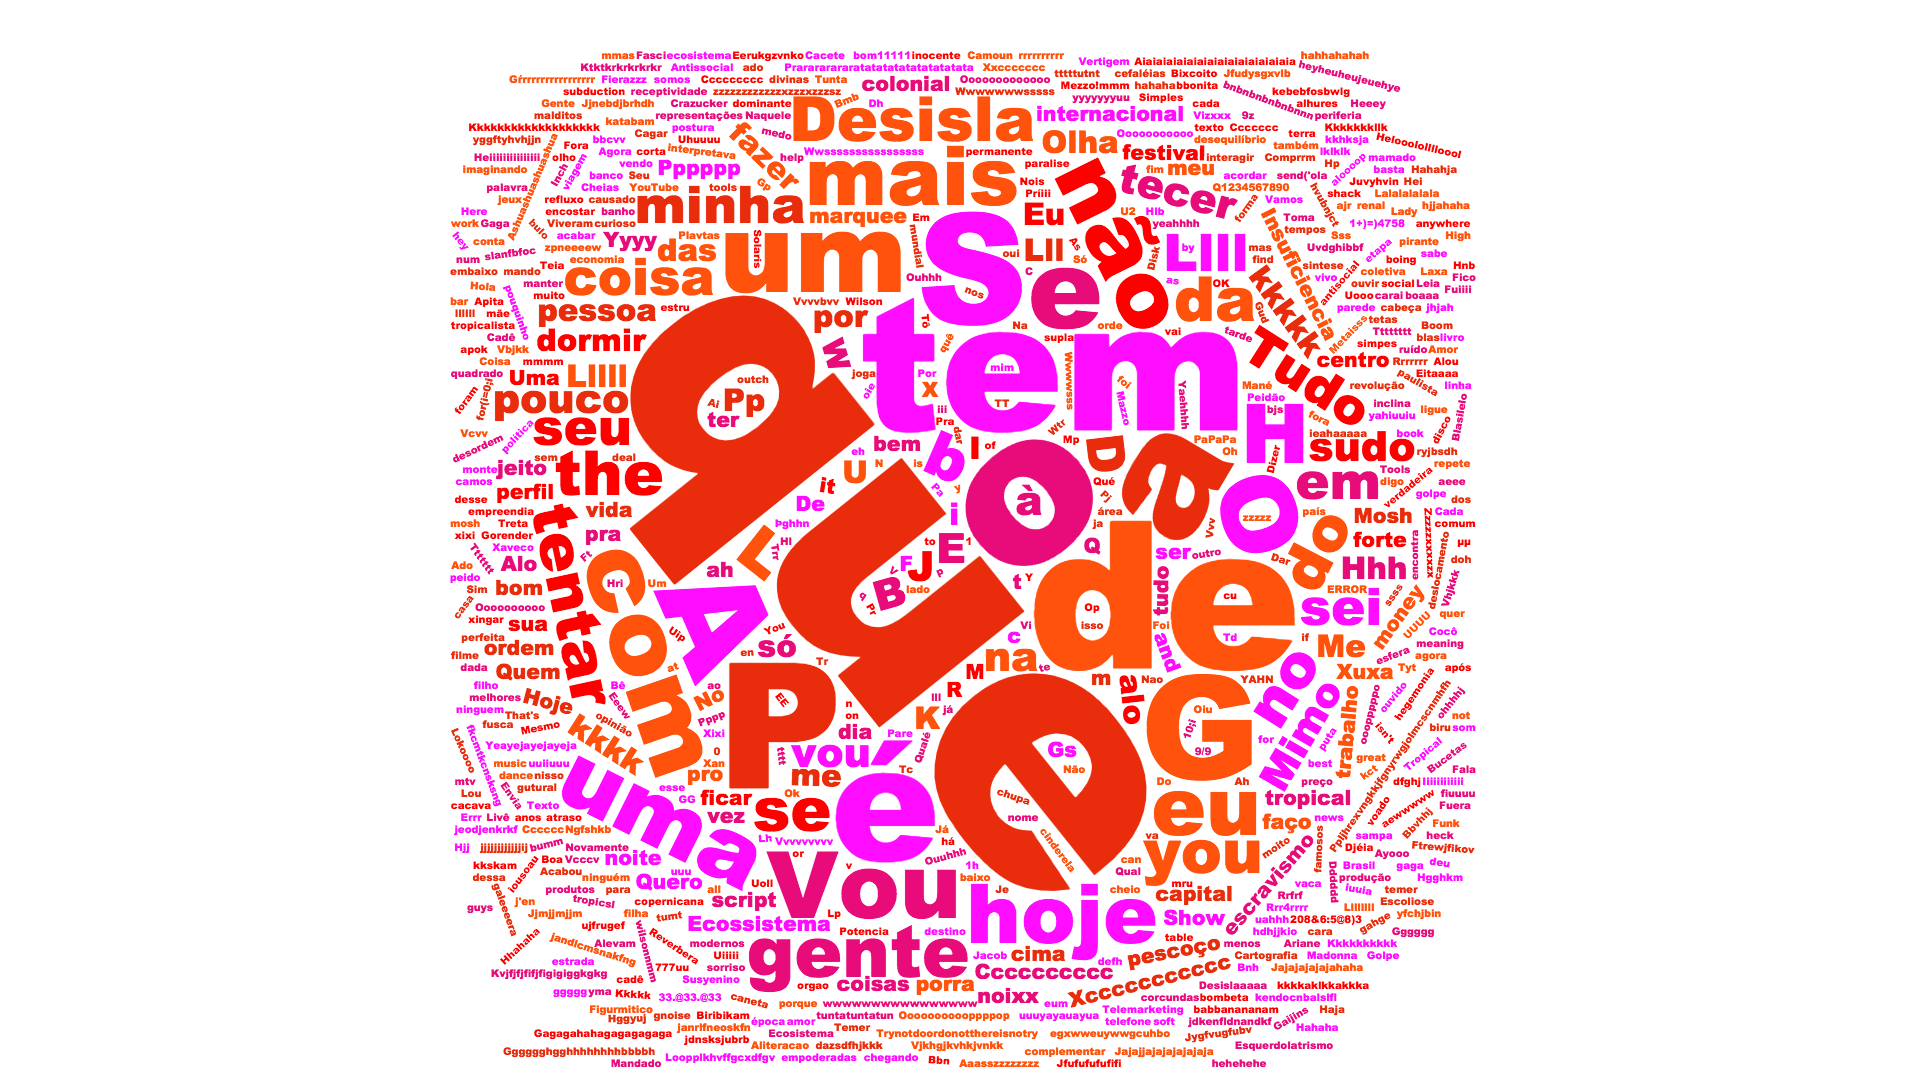
\includegraphics[width=1\linewidth]{img/wordcloud_performance4.png}
\caption{Tag cloud of the performance 4.}
\end{figure}


\begin{figure*}
\centering
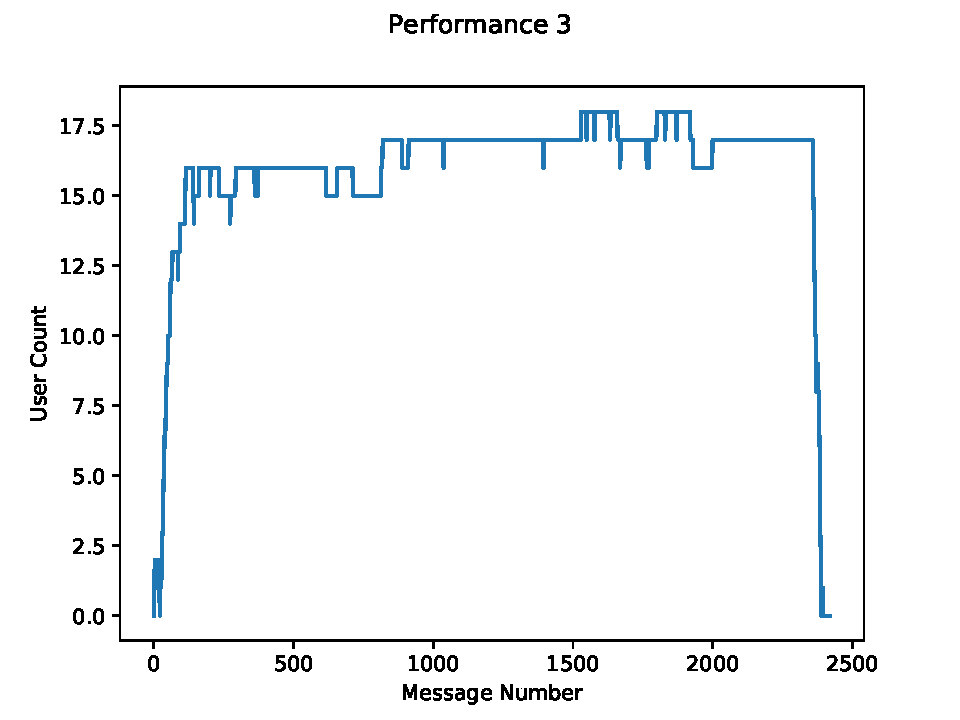
\includegraphics{num_analysis/p3_us.pdf}
\caption{User count for the third performance. The x-axis represents the message number in the log.}
\end{figure*}

\subsection{Overall data}

\begin{figure*}
\centering
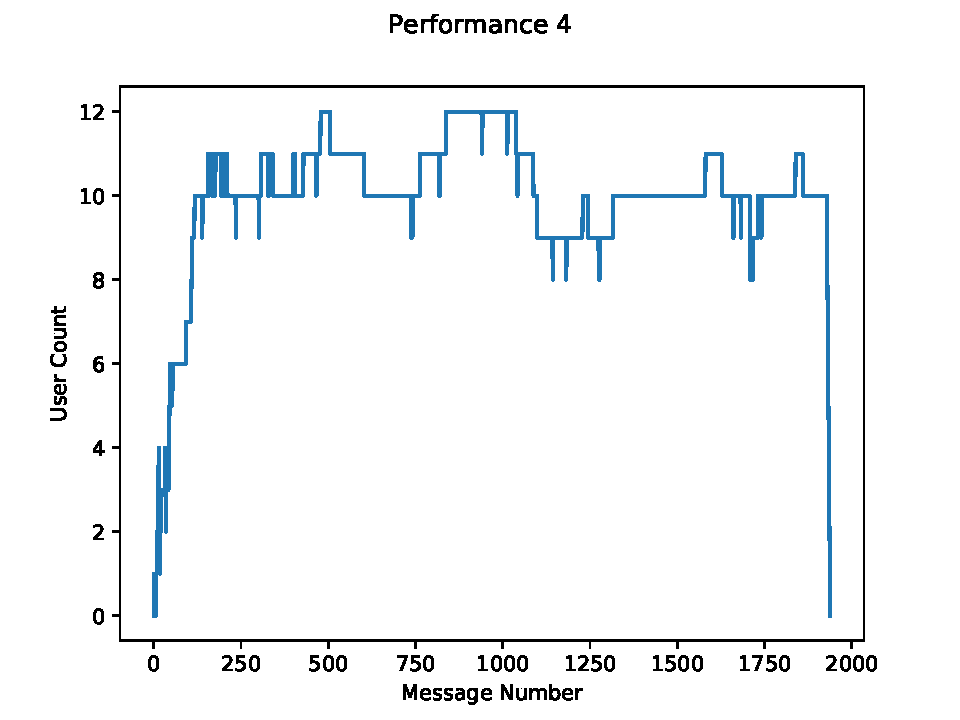
\includegraphics{num_analysis/p4_us.pdf}
\caption{User count for the fourth performance. The x-axis represents the message number in the log.}
\end{figure*}

%Table

%\tbl{}{%
%\begin{tabular}{@{}lcccc@{}}\toprule

Over those performances, there were 7145 messages that users intentionally have written. There were 865 unique sessions, a session created everytime a person loads the page. This means, on average, a user would send 8.26 messages per session.

\begin{table}
\tabcolsep8.1pt
\tbl{Quantitative data about the performances}{%
\begin{tabular}{@{}lc@{}}\toprule
 Number of written messages & 7145\\
 Number of unique sessions & 865\\
 Number of maximum simultaneous users & 31\\
 Average number of messages for unique session & 8.26\\\botrule
\end{tabular}}
\begin{tabnote}
Quantitative data about the performance.
\end{tabnote}
\end{table}

number of unique participants
average number of message/participant

text statistics

number of messages for sample pack

average size of messages
number of messages/size

most used tokens
number of unique tokens

meaningful tokens
emoticons and special characters  


\section{Background}


%Head 2
\subsection{Chirp-Like Impulse Responses and Group Delay}


%Head 3
\subsubsection{Chirp-Like Impulse Responses and Group Delay}

%Equation
\begin{equation}
A(z) = \frac{{a_1  + z^{ - 1} }}{{1 + a_1 z^{ - 1} }},
\end{equation}




                              

\begin{equation}
\tau _{\textrm{g,max}}  = \left\{ \begin{array}{l}
 \tau _\textrm{g} (0) = \frac{{1 - a_1 }}{{1 + a_1 }},\textrm{when }a_1  \le 0 \\[4pt]
 \tau _\textrm{g} (\pi ) = \frac{{1 + a_1 }}{{1 - a_1 }},\textrm{when }a_1  > 0. \\
 \end{array} \right.\end{equation}

The phonetic alphabet was as pointed McLuhan \cite{mcluhan_understanding_1964}, a fundamental technology for the developing our culture, by giving power to authority at distance, been it's easy to learn and adjustable to many languages, and base for all literacy. Here we are trying to make use of the alphabet as technology to produce experimental music. Since text messages are probably the main form of communication on smartphones today, we choose to experiment possibilities to experiment with type as input to produce interactive music. Many kinds of interfaces uses typing as input, through text, such as in live coding \cite{Collins2003live} and audience participation pieces, to receive feedback \cite{noauthor_transglasphone_nodate} or get user data as source for algorithm compositions [8] or using keyboard as music controllers \cite{fiebrink_dont_2007}.

we proposed an interface that could work by typing



%Paragraph listing
%\begin{paralist}
%\item{}Filtering an audio signal with an allpass filter does not usually have a major effect on the signal's timbre. The allpass filter does not change the frequency content of the signal, but only introduces a phase shift or delay. 
%\item{}Audibility of the phase distortion caused by an allpass filter in a sound reproduction system has been a topic of many studies, see, e.g.. 
%\item{}In this paper, we investigate audio effects processing using high-order allpass filters that consist of many cascaded low-order allpass filters. These filters have long chirp-like impulse responses. 
%\end{paralist}

%Interaction process happens through an open chat interface (see figure 1), where there is no distinction between users, so no one can tell who is playing what; each message sent to the chat is loaded into chat room and played as a sequence of samples with no hierarchy; in an inter-semiotic translation \cite{plaza1987traduccao}, we decode the text messages in musical information, through concatenation of samples. To touch or click in the messages on screen makes them to play again. Unlike speech synthesis mechanism, our sound chat does not concatenate syllables, so words cannot be understood as words, but only as sound rhythmic sequences; as people join the conversation, the rhythm becomes more frenetic and the sound layer becomes more dense and entropic. 
%Besides the sound that comes from people typing, there are also commands that can be live coded. Those commands are hidden from the public creating some degree of surprise. They can change the audio samples pack or change the global volumes and turn off the sound. In the last version of the software it's possible to establish a BPM tempo for the samples being played.




%Figure
%\begin{figure}
%\centering
%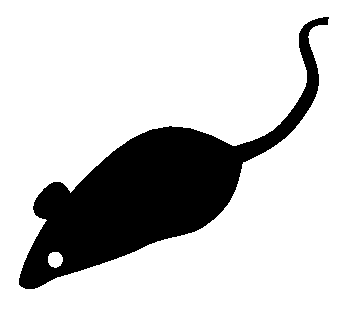
\includegraphics{aes2e-mouse.eps}
%\caption{The spectral delay filter consists of \textit{M} allpass filters and an equalization filter.}
%\end{figure}


%\begin{figure*}
%\centering
%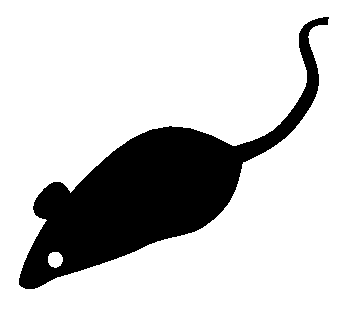
\includegraphics[width=23pc]{aes2e-mouse.eps}
%\caption{This paper is organized as follows. In Section 1, we discuss the group delay of a cascade of first-order allpass filters and its relation to the chirp-like impulse response of the spectral delay filter. Furthermore, a multirate method to stretch the impulse response of the spectral delay filter is proposed. Section 2 discusses the amplitude envelope of the impulse response and suggests a design method for the equalizing filter. Section 3 presents application examples using the spectral delay filter. Section 4 concludes this paper.}
%\end{figure*}
%Filtering an audio signal with an allpass filter does not usually have a major effect on the signal's timbre. The allpass filter does not change the frequency content of the signal, but only introduces a phase shift or delay.

\begin{extract}

%\begin{alphalist}
%\item{}Green--function determined experimentally and published.
%\item{}Black--function determined using similarity searches and published.
%\item{}Red--function determined using similarity searches and determined in this study.
%\item{}Blue--O-antigen structure unknown. Function determined using similarity searches and proposed in this study.
%\end{alphalist}

%Enunciations
%\begin{bulletlist}
%\item{}Green--function determined experimentally and published.
%\item{}Black--function determined using similarity searches and published.
%\item{}Red--function determined using similarity searches and determined in this study.
%\item{}Blue--O-antigen structure unknown. Function determined using similarity searches and proposed in this study.
%\end{bulletlist}

%\begin{unnumlist}
%\item{}Green--function determined experimentally and published.
%\item{}Black--function determined using similarity searches and published.
%\item{}Red--function determined using similarity searches and determined in this study.
%\item{}Blue--O-antigen structure unknown. Function determined using similarity searches and proposed in this study.
%\end{unnumlist}


\section{SUMMARY}


\section{CONCLUSION}
Joy is the real proof - manifesto antropófago
For be more open, users should be able to map sound into letters, so we are proposing to use freesound API to map sounds into letters. We are corrent developing an interface to search sounds with the freesound api 


\section{ACKNOWLEDGMENT}
This project was developed with the support of the NuSom  - Research Centre on Sonology at the University of São Paulo and C4DM - Centre for Digital Music at Queen Mary University of London.

This research was conducted in fall 2008 when Vesa V\"alim\"aki was a visiting scholar at CCRMA, Stanford University. His visit was financed by the Academy of Finland (project no. 126310). The authors would like to Dr. Henri Penttinen for his comments and for the snare drum sample used in this work.

\bibliography{aes2e.bib}
\bibliographystyle{aes2e.bst}

% NOTE:
% - in case you are not using bibTex you have to manually edit the bibliograpy as below.
% - if submitting a bibTex file is not allowed you can copy the content from the aes2e.bbl file  
\begin{thebibliography}{99}
%
%\newcommand{\enquote}[1]{``#1''}
%\providecommand{\url}[1]{\texttt{#1}}
%\providecommand{\urlprefix}{URL }
%\expandafter\ifx\csname urlstyle\endcsname\relax
%  \providecommand{\doi}[1]{[Online]. Available: \discretionary{}{}{}#1}\else
%  \providecommand{\doi}{doi:\discretionary{}{}{}\begingroup
%  \urlstyle{rm}\Url}\fi
%
%\bibitem{DEK1}
%D.~Preis, \enquote{Phase Distortion and Phase Equalization in Audio Signal
%  Processing---A Tutorial Review,} \emph{J. Audio Eng. Soc.}, vol.~30, no.~11,
%  pp. 774--779 (1982 Nov.).
%
%\bibitem{DEK2}
%J.~S. Abel, D.~P. Berners, \enquote{MUS424/EE367D: Signal Processing Techniques
%  for Digital Audio Effects,}  (2005), unpublished Course Notes, CCRMA,
%  Stanford University, Stanford, CA.
%
%\bibitem{DEK3}
%C.~Roads, \enquote{Musical Sound Transformation by Convolution,} presented at
%  the \emph{Int. Computer Music Conf.}, pp. 102--109 (1993).
%
%\bibitem{DEK4}
%C.~Roads, \emph{The Computer Music Tutorial} (MIT Press, Cambridge, MA), 1st
%  ed. (1996).
%
%\bibitem{DEK5}
%H.~Morgenstern, B.~Rafaely, \enquote{Spatial Reverberation and Dereverberation
%  Using an Acoustic Multiple-Input Multiple-Output System,} \emph{J. Audio Eng.
%  Soc}, vol.~65, no. 1/2, pp. 42--55 (2017 Jan.Feb.),
%  \doi{https://doi.org/10.17743/jaes.2016.0063}.
%  
\end{thebibliography}

%Appendix
\appendix
\section*{APPENDIX}
%Filtering an audio signal with an allpass filter does not usually have a major effect on the signal's timbre. The allpass filter does not change the frequency content of the signal, but only introduces a phase shift or delay. Audibility of the phase distortion caused by an allpass filter in a sound reproduction system has been a topic of many studies, see, e.g., \cite{DEK1}, \cite{DEK2}.
\begin{equation}
\phi (\omega ) =  - \omega  + 2\arctan \left( {\frac{{a_1 \sin \omega }}{{1 + a_1 \cos \omega }}} \right)
\end{equation}

In this paper, we investigate audio effects processing using high-order allpass filters that consist of many cascaded low-order allpass filters. These filters have long chirp-like impulse responses. When audio and music signals are processed with such a filter, remarkable changes are obtained that are similar to the spectral delay effect  \cite{DEK3}, \cite{DEK4}.


\begin{nomenclature}[PAMPs]
\subsection*{NOMENCLATURE}
\nomentry{a$_c$}{condensation coefficient condensation coefficient condensation coefficient}


\nomentry{TLR}{Toll-like receptor}

\nomentry{PAMPs}{pathogen-associated molecular patterns condensation coefficient condensation}
\end{nomenclature}

%Biography
 \biography{A1firstname A1lastname}{a.eps}{A1firstname A1lastname is professor of audio signal processing at Helsinki University of Technology (TKK), Espoo, Finland. He received his Master of Science in Technology, Licentiate of Science in Technology, and Doctor of Science in Technology degrees in electrical engineering from TKK in 1992, 1994, and 1995, respectively. His doctoral dissertation dealt with fractional delay filters and physical modeling of musical wind instruments. Since 1990, he has worked mostly at TKK with the exception of a few periods. In 1996 he spent six months as a postdoctoral research fellow at the University of Westminster, London, UK. In 2001-2002 he was professor of signal processing at the Pori School of Technology and Economics, Tampere University of Technology, Pori, Finland. During the academic year 2008-2009 he has been on sabbatical and has spent several months as a visiting scholar at the Center for Computer Research in Music and Acoustics (CCRMA), Stanford University, Stanford, CA. His research interests include musical signal processing, digital filter design, and acoustics of musical instruments. Prof. V\"alim\"aki is a senior member of the IEEE Signal Processing Society and is a member of the AES, the Acoustical Society of Finland, and the Finnish Musicological Society. He was the chairman of the 11th International Conference on Digital Audio Effects (DAFx-08), which was held in Espoo, Finland, in 2008.}
 \biography{A2firstname A2lastname}{b.eps}{A2firstname A2lastname is a consulting professor at the Center for Computer Research in Music and Acoustics (CCRMA) in the Music Department at Stanford University where his research interests include audio and music applications of signal and array processing, parameter estimation, and acoustics. From 1999 to 2007, Abel was a co-founder and chief technology officer of the Grammy Award-winning Universal Audio, Inc. He was a researcher at NASA/Ames Research Center, exploring topics in room acoustics and spatial hearing on a grant through the San Jose State University Foundation. Abel was also chief scientist of Crystal River Engineering, Inc., where he developed their positional audio technology, and a lecturer in the Department of Electrical Engineering at Yale University. As an industry consultant, Abel has worked with Apple, FDNY, LSI Logic, NRL, SAIC and Sennheiser, on projects in professional audio, GPS, medical imaging, passive sonar and fire department resource allocation. He holds Ph.D. and M.S. degrees from Stanford University, and an S.B. from MIT, all in electrical engineering. Abel is a Fellow of the Audio Engineering Society.}
\end{extract} 
\end{document}